\section{Présentation du sujet} % Pas de numérotation
\addcontentsline{toc}{section}{Présentation du sujet} % Ajout dans la table des matières

\subsection{Un rapide résumé}
Le logiciel MovieManager est un gestionnaire de films permettant de gérer les films vus par l'utilisateur, de charger une base de films à partir d'un fichier texte, de les exporter en format json, et de créer une liste de propositions de films à voir.

\begin{figure}[!ht]
    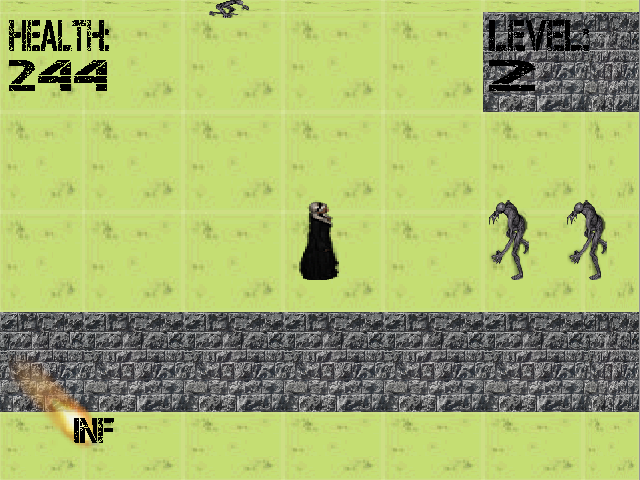
\includegraphics[width=0.5\textwidth]{./images/snapshot1.png}
    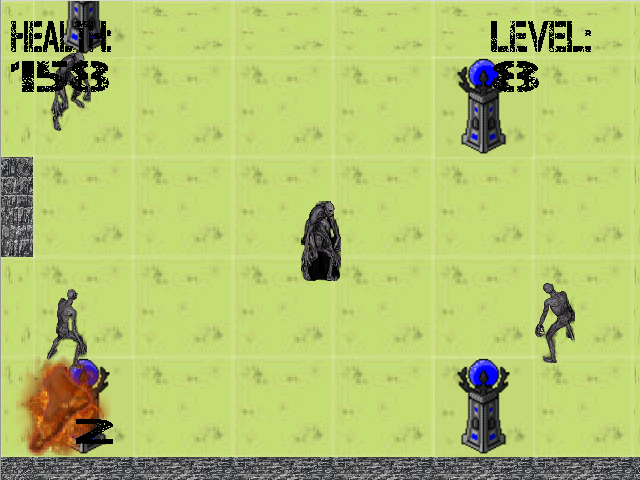
\includegraphics[width=0.5\textwidth]{./images/snapshot2.png}
    \caption{Captures d'écran}
\end{figure}

Nous n'avons pas inclus de vue en console, mais uniquement une vue graphique. En effet, après demande de renseignements, on nous a dit qu'il n'était pas nécessaire de l'implémenter.

\subsection{Les objectifs recherchés}
Le but du programme est d'établir un standard de films qui correspond aux goûts de l'utilisateur. Une fois ce standard défini, nous recherchons dans le modèle les films qui lui sont proches. Ainsi, on ne proposera pas forcément les suites de films déjà vus par l'utilisateur si lesdits films ne font pas partie de ses films les plus regardés. \\
Dans le calcul de la distance entre les films, toutes les composantes sont prises en compte. On leur attribue des poids définis arbitrairement. Ainsi, voici leur hiérarchie :

\begin{itemize}
	\item Titre du film
	\item Liste des genres
	\item Réalisateur
	\item Liste des acteurs
	\item Type (Film ou série TV)
\end{itemize}

